\documentclass[10pt,x11names,table]{beamer}

\usetheme[progressbar=frametitle]{metropolis}
\usepackage{appendixnumberbeamer}
\usepackage{xcolor}

\usepackage{polyglossia}
\setmainlanguage{spanish}

\usepackage{listings}

\usepackage{booktabs}
\usepackage[scale=2]{ccicons}

\usepackage{pgfplots}
\usepgfplotslibrary{dateplot}

%ANIMACIONES
\usepackage{animate}
\usepackage{graphicx}
\usepackage[caption=false]{subfig}

\usepackage{xspace}

\newcommand*{\eg}{e.g.\@\xspace}
\newcommand*{\ie}{i.e.\@\xspace}

\let\oldquote\quote
\let\endoldquote\endquote
\renewenvironment{quote}[2][]
  {\if\relax\detokenize{#1}\relax
     \def\quoteauthor{#2}%
   \else
     \def\quoteauthor{#2~---~#1}%
   \fi
   \oldquote}
  {\par\nobreak\smallskip\hfill(\quoteauthor)%
   \endoldquote\addvspace{\bigskipamount}}
   
\usepackage{wrapfig}

\usepackage{subfig}
\usepackage{hyperref}
\usepackage{multicol}

\setbeamertemplate{bibliography item}[text]

\usepackage[font=small,skip=0pt, labelformat=empty]{caption}

\usepackage{dirtytalk}
\usepackage[acronym]{glossaries}
\makeglossaries

\newacronym{acgan}{ACGAN}{Auxiliary Classifier GAN}
\newacronym{ae}{AE}{Autoencoder}
\newacronym{ai}{AI}{Artificial Intelligence}
\newacronym{api}{API}{Application Programming Interface}
\newacronym{bert}{BERT}{Bidirectional Encoder Representations from Transformers}
\newacronym{brief}{BRIEF}{Binary Robust Independent Elementary Features}
\newacronym{brnn}{BRNN}{Bidirectional RNN}
\newacronym{bptt}{BPTT}{Backpropagation Through Time}
\newacronym{cbow}{CBOW}{Continous bag-of-words}
\newacronym{cnn}{CNN}{Convolutional Neural Network}
\newacronym{crnn}{CRNN}{Convolutional Recurrent Neural Network}
\newacronym{ddpm}{DDPM}{Denoising Diffusion Probabilistic Model}
\newacronym{ddim}{DDIM}{Denoising Diffusion Implicit Model}
\newacronym{diffit}{DiffiT}{Diffusion Vision Transformer}
\newacronym{dl}{DL}{Deep Learning}
\newacronym{dnn}{DNN}{Deep Neural Network}
\newacronym{dos}{DoS}{Denial of Service}
\newacronym{drnn}{DRNN}{Deep Recurrent Neural Network}
\newacronym{ecg}{ECG}{Electrocardiogram}
\newacronym{elmo}{ELMo}{Embedding from Language Model}
\newacronym{fast}{FAST}{Features from Accelerated Segment Test}
\newacronym{fid}{FID}{Fréchet Inception Distance}
\newacronym{foss}{FOSS}{Free and open-source software}
\newacronym{gan}{GAN}{Generative Adversarial Network}
\newacronym{glove}{GloVe}{Global Vectors for Word Representation}
\newacronym{gpu}{GPU}{Graphics Processing Unit}
\newacronym{gru}{GRU}{Gated Recurrent Unit}
\newacronym{ilsvrc}{ILSVRC}{ImageNet Large Scale Visual Recognition Challenge}
\newacronym{is}{IS}{Inception Score}
\newacronym{kid}{KID}{Kernel Inception Distance}
\newacronym{ldm}{LDM}{Latent Diffusion Model}
\newacronym{lstm}{LSTM}{Long Short-Term Memory}
\newacronym{mape}{MAPE}{Mean Absolute Perentage Error}
\newacronym{ml}{ML}{Machine Learning}
\newacronym{mlp}{MLP}{Multilayer Perceptron}
\newacronym{mmd}{MMD}{Maximum Mean Discrepancy}
\newacronym{mse}{MSE}{Mean Squared Error}
\newacronym{ner}{NER}{Named Entity Recognition}
\newacronym{nlg}{NLG}{Natural Language Generation}
\newacronym{nlp}{NLP}{Natural Language Processing}
\newacronym{nlu}{NLU}{Natural Language Understanding}
\newacronym{nn}{NN}{Neural Network}
\newacronym{ocr}{OCR}{Optical Character Recognition}
\newacronym{onnx}{ONNX}{Open Neural Network Exchange}
\newacronym{pmml}{PMML}{Predictive Model Markup Language}
\newacronym{relu}{ReLU}{Rectified Linear Unit}
\newacronym{rest}{REST}{Representational State Transfer}
\newacronym{rnn}{RNN}{Recurrent Neural Network}
\newacronym{sae}{SAE}{Stacked Autoencoder}
\newacronym{sift}{SIFT}{Scale-Invariant Feature Transform}
\newacronym{slam}{SLAM}{Simultaneous Localization and Mapping}
\newacronym{sru}{SRU}{Single Recurrent Unit}
\newacronym{surf}{SURF}{Speeded-Up Robust Features}
\newacronym{svm}{SVM}{Support Vector Machine}
\newacronym{vae}{VAE}{Variational Autoencoder}
\newacronym{vgg}{VGG}{Visual Geometry Group}
\newacronym{vit}{ViT}{Vision Transformer}
\newacronym{wsgi}{WSGI}{Web Server Gateway Interface}
\newacronym{xai}{XAI}{eXplainable Artificial Intelligence}
\newacronym{yolo}{YOLO}{You Only Look Once}
\newacronym{zsl}{ZSL}{Zero-shot Learning}
\subtitle{Métodos Generativos, curso 2024-2025}

\date{\today}
\author{Guillermo Iglesias, guillermo.iglesias@upm.es \newline
Jorge Dueñas Lerín, jorge.duenas.lerin@upm.es  \newline
Félix Fuentes Hurtado, felix.fuentes@upm.es}

\institute{Escuela Técnica Superior de Ingeniería de Sistemas Informáticos | UPM \newline
\hbox{} \newline \ccbysa \hspace{0.1pt} \ccNonCommercial}

%%%%%%%%%%%%%%%%%%%%%%%%%%%%%%%%%%%%%       
\title{Presentación de la asignatura}

\begin{document}
\maketitle

\begin{frame}{Motivación}
En esta asignatura veremos qué son los \alert{modelos generativos} y qué se puede hacer con ellos.

Será una asignatura eminentemente \alert{práctica}.

El objetivo es desarrollar las habilidades necesarias para poder hacer uso práctico de cualquier tipo de método generativo, entendiendo, para ello,

\centering
\alert{\huge la teoría que los sustenta}.
\end{frame}

\begin{frame}{Profesorado}

\begin{columns}[T]
\begin{column}{.98\textwidth}
\centering
\alert{\Large Félix Fuentes Hurtado (\textbf{Coordinador})}

({\color{blue}felix.fuentes@upm.es})

Despacho 4305.
\end{column}
\end{columns}

\hfill

\begin{columns}[T]
\begin{column}{.49\textwidth}
\alert{\Large Guillermo Iglesias Hernández}

({\color{blue}guillermo.iglesias@upm.es})

Despacho 1306.
\end{column}
\hfill
\begin{column}{.49\textwidth}
\alert{\Large Jorge Dueñas Lerín}

({\color{blue}jorge.duenas.lerin@upm.es})

Despacho 4215.
\end{column}
\end{columns}
\end{frame}

\begin{frame}{Presentación del alumnado}
\centering \alert{\Large Vuestro turno!}
\begin{figure}
    \centering
    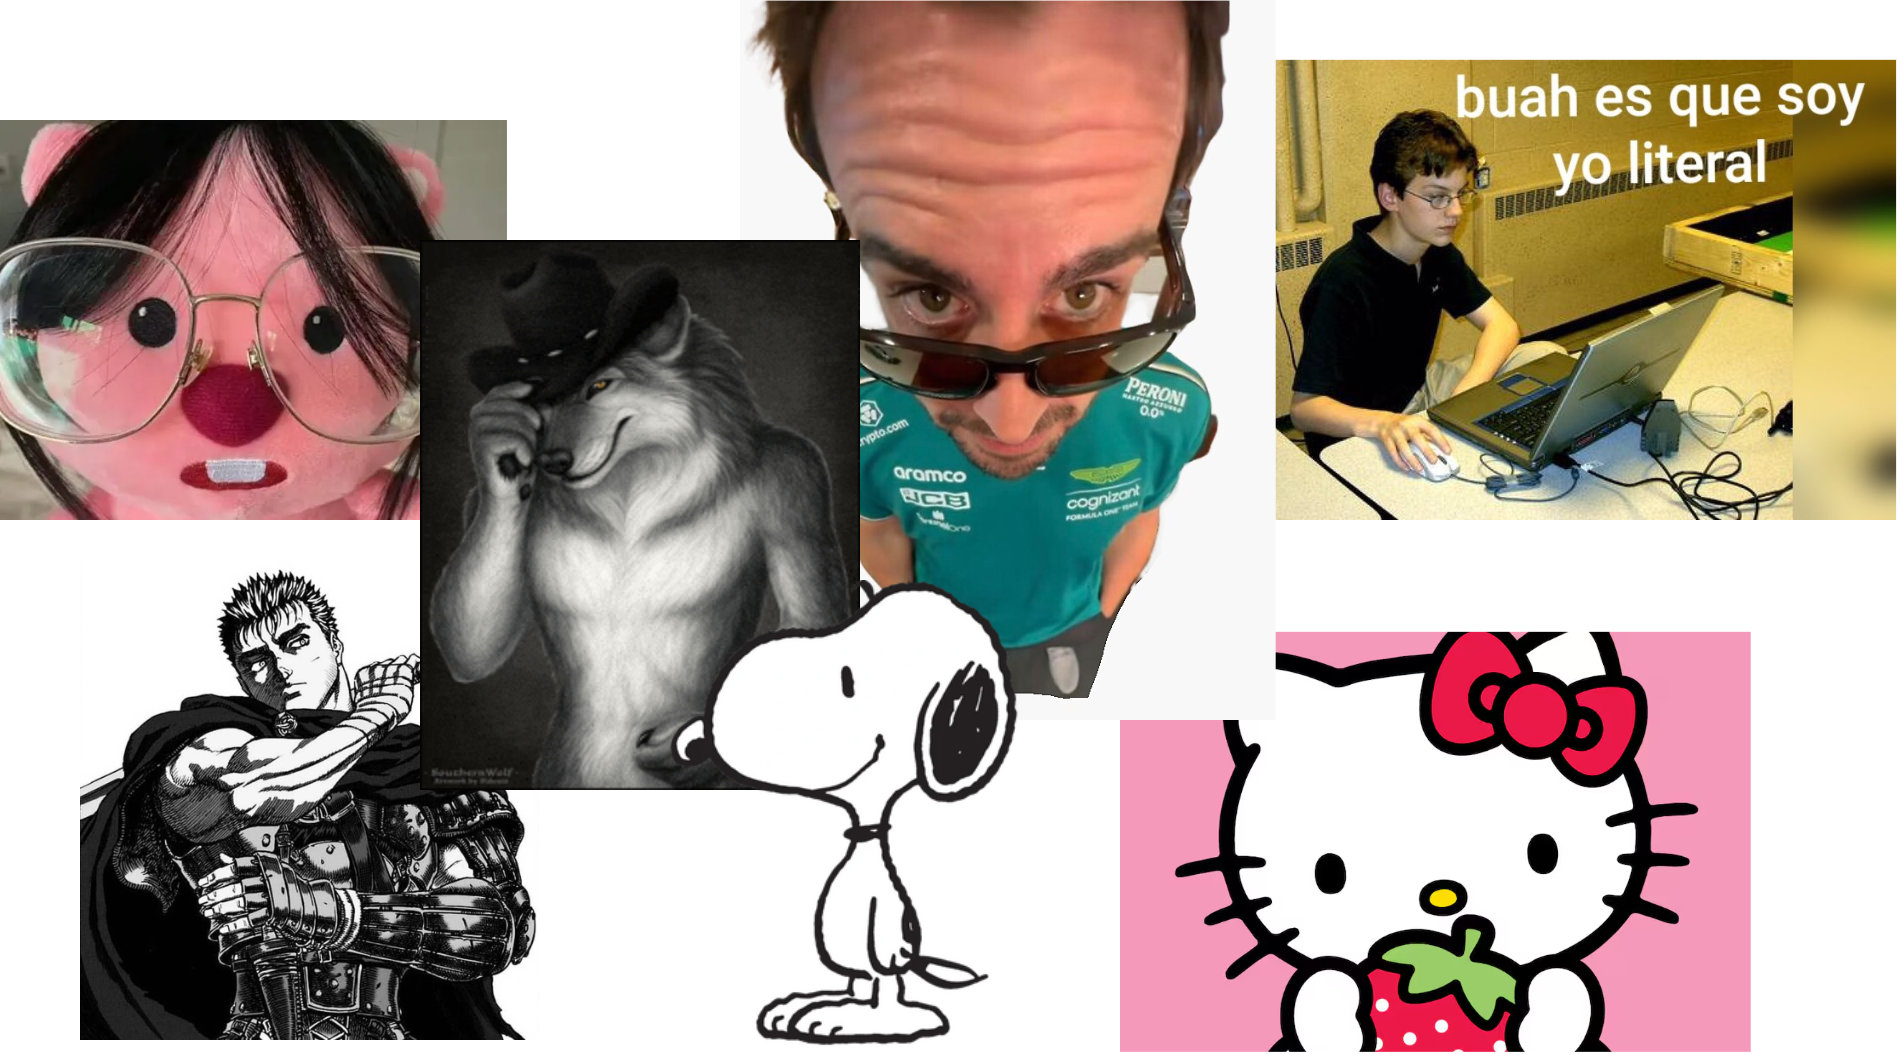
\includegraphics[width=\textwidth]{Slides/figures/Presentacion/Presentacion_Alumnos.png}
\end{figure}
\end{frame}

\begin{frame}[allowframebreaks]{Temario de la asignatura}
\alert{\Large Tema 1. Introducción.}
\begin{itemize}
\item Redes neuronales.
\item Redes neuronales convolucionales.
%\item Aplicaciones de redes convolucionales.
\end{itemize}

\alert{\Large Tema 2. Arquitecturas de métodos generativos.}
\begin{itemize}
\item Introducción a los métodos generativos.
\item Autoencoders (AE).
\item Autoencoders variacionales (VAE).
\item Generative Adversarial Networks (GAN).
\item Transformers.
\item Diffusion Models.
\end{itemize}

\framebreak

\alert{\Large Tema 3. Aplicaciones prácticas.}
\begin{itemize}
\item Aplicaciones prácticas (texto).
\item Aplicaciones prácticas (imagen).
\end{itemize}

\alert{\Large Tema 4. Práctica libre grupal.}
\end{frame}


\begin{frame}{Criterios de calificación}
\alert{\Large Evaluación progresiva.}
\begin{itemize}
    \item 2 exámenes (\alert{\textbf{40\%}}).
    \item 3 prácticas individuales (\alert{\textbf{30\%}}).
    \item 1 práctica grupal (\alert{\textbf{30\%}}).
\end{itemize}

\alert{\Large Evaluación global.}
\begin{itemize}
    \item 1 examen (\alert{\textbf{100\%}}).
    \begin{itemize}
        \item Nota mínima \textbf{5/10}.
    \end{itemize}
\end{itemize}

\alert{\Large Evaluación extraordinaria.}
\begin{itemize}
    \item 1 examen (\alert{\textbf{100\%}}).
    \begin{itemize}
        \item Nota mínima \textbf{5/10}.
    \end{itemize}
\end{itemize}
\end{frame}

\begin{frame}{Criterios de evaluación progresiva}
\begin{columns}[T]
\begin{column}{.49\textwidth}
Exámenes.
\end{column}
\hfill
\begin{column}{.49\textwidth}
\centering
\alert{\Huge 40\%}
\end{column}
\end{columns}
\vfill
\hrule

\begin{itemize}
    \item Examen 1: Temas 1 y 2 (\alert{20\%})
    \item Examen 2: Tema 3 (\alert{20\%})
\end{itemize}
\vfill
\hrule
\hrule

\vfill
\begin{columns}[T]
\begin{column}{.49\textwidth}
\vspace{0.2cm}
Prácticas individuales.
\end{column}
\hfill
\begin{column}{.49\textwidth}
\centering
\alert{\Huge 30\%}
\end{column}
\end{columns}
\vfill
\hrule

\begin{itemize}
    \item Práctica 1: Autoencoders (\alert{10\%}).
    \item Práctica 2: GANs (\alert{10\%}).
    \item Práctica 3: Transformers (\alert{10\%}).
\end{itemize}
\vfill

\hrule
\hrule

\vfill
\begin{columns}[T]
\begin{column}{.49\textwidth}
\vspace{0.2cm}
Práctica final grupal.
\end{column}
\begin{column}{.49\textwidth}
\centering
\alert{\Huge 30\%}
\end{column}
\end{columns}
\end{frame}

\begin{frame}{Criterios de evaluación global y extraordinaria}
\begin{columns}[T]
\begin{column}{.49\textwidth}
\vfill
Examen final.
\vfill
\end{column}

\begin{column}{.49\textwidth}
\centering
\vfill
\alert{\Huge 100\%}
\vfill
\end{column}
\end{columns}
\vfill
\hrule
\vfill

\begin{itemize}
    \item Temas 1, 2 y 3 (\alert{100\%})\footnote{La \alert{nota mínima} del examen final será de \alert{5/10}}
\end{itemize}
\vfill

\end{frame}

\begin{frame}{Criterios de calificación}
Ninguna de las prácticas o cuestionarios es recuperable. \alert{La no realización, o realización en blanco, de una práctica o cuestionario será calificado con un 0 en la nota final}.
\begin{itemize}
    \item \alert{Exámenes teóricos}: Consistirá en una prueba por escrito con el objetivo de evaluar los conocimientos teóricos del alumno de cada uno de los temas.
    \item \alert{Prácticas individuales}: Pruebas para poner en práctica los conocimientos adquiridos en los distintos temas de la asignatura.
\end{itemize}
\end{frame}

\begin{frame}{Criterios de calificación}
Los grupos de la \alert{práctica grupal} final serán de \alert{3 personas}.

El \alert{resto} de prácticas serán \alert{individuales}.

Aquellos que lo deseen podrán presentarse a la \alert{evaluación global}. Para ello, tendrán que notificar de dicha elección al coordinador de la asignatura.
\end{frame}

\begin{frame}{Normas}
\begin{itemize}
    \item Las actividades hay que \alert{entregarlas antes} de la fecha límite.
    \item \alert{Respetar} a los compañeros y a su derecho a la educación.
    \item \alert{Citar} claramente todas las fuentes (incluidos colaboradores).
    \begin{itemize}
        \item Así mantenemos una correcta ética de trabajo.
        \item Ayuda a la evolución de la asignatura y los futuros estudiantes lo agradecerán.
    \end{itemize}
    \item La colaboración con otros humanos se debería \alert{limitar a discusión}.
    \begin{itemize}
        \item El código y la documentación deberá realizarla el grupo o individuo responsable de la práctica.
        \item Cada estudiante debe ser capaz de responder a cuantas preguntas se le hagan sobre sus tareas cuando se le solicite
    \end{itemize}
    \item Se mantiene una \alert{tolerancia cero} ante el \alert{plagio}.
    \begin{itemize}
        \item Cualquier plagio detectado implicará un suspenso en la convocatoria actual.
    \end{itemize}
\end{itemize}
\end{frame}

\begin{frame}{Código de conducta \cite{ConductCode}}
Se requiere que estudiantes y docentes acepten el siguiente código de conducta. La coordinación de la asignatura hará cumplir este código a lo largo del curso. Esperamos la colaboración de todos los participantes para ayudar a asegurar un ambiente seguro.

Esta asignatura pretende ofrecer una experiencia \alert{libre de abusos} para todas las personas, independientemente de su género, orientación sexual, discapacidad, apariencia física, talla, raza o religión. \alert{No toleramos abusos en ninguna de sus formas}. El lenguaje e imágenes abusivos no son apropiados para ningún ámbito de la asignatura, incluidas diapositivas, trabajos entregados, comentarios en Moodle, X/Twitter y otros medios online. Las personas que violen estas reglas pueden ser \alert{sancionadas o expulsadas de las clases o exámenes}.
\end{frame}

\begin{frame}{Calendario académico}
\begin{figure}
    \centering
    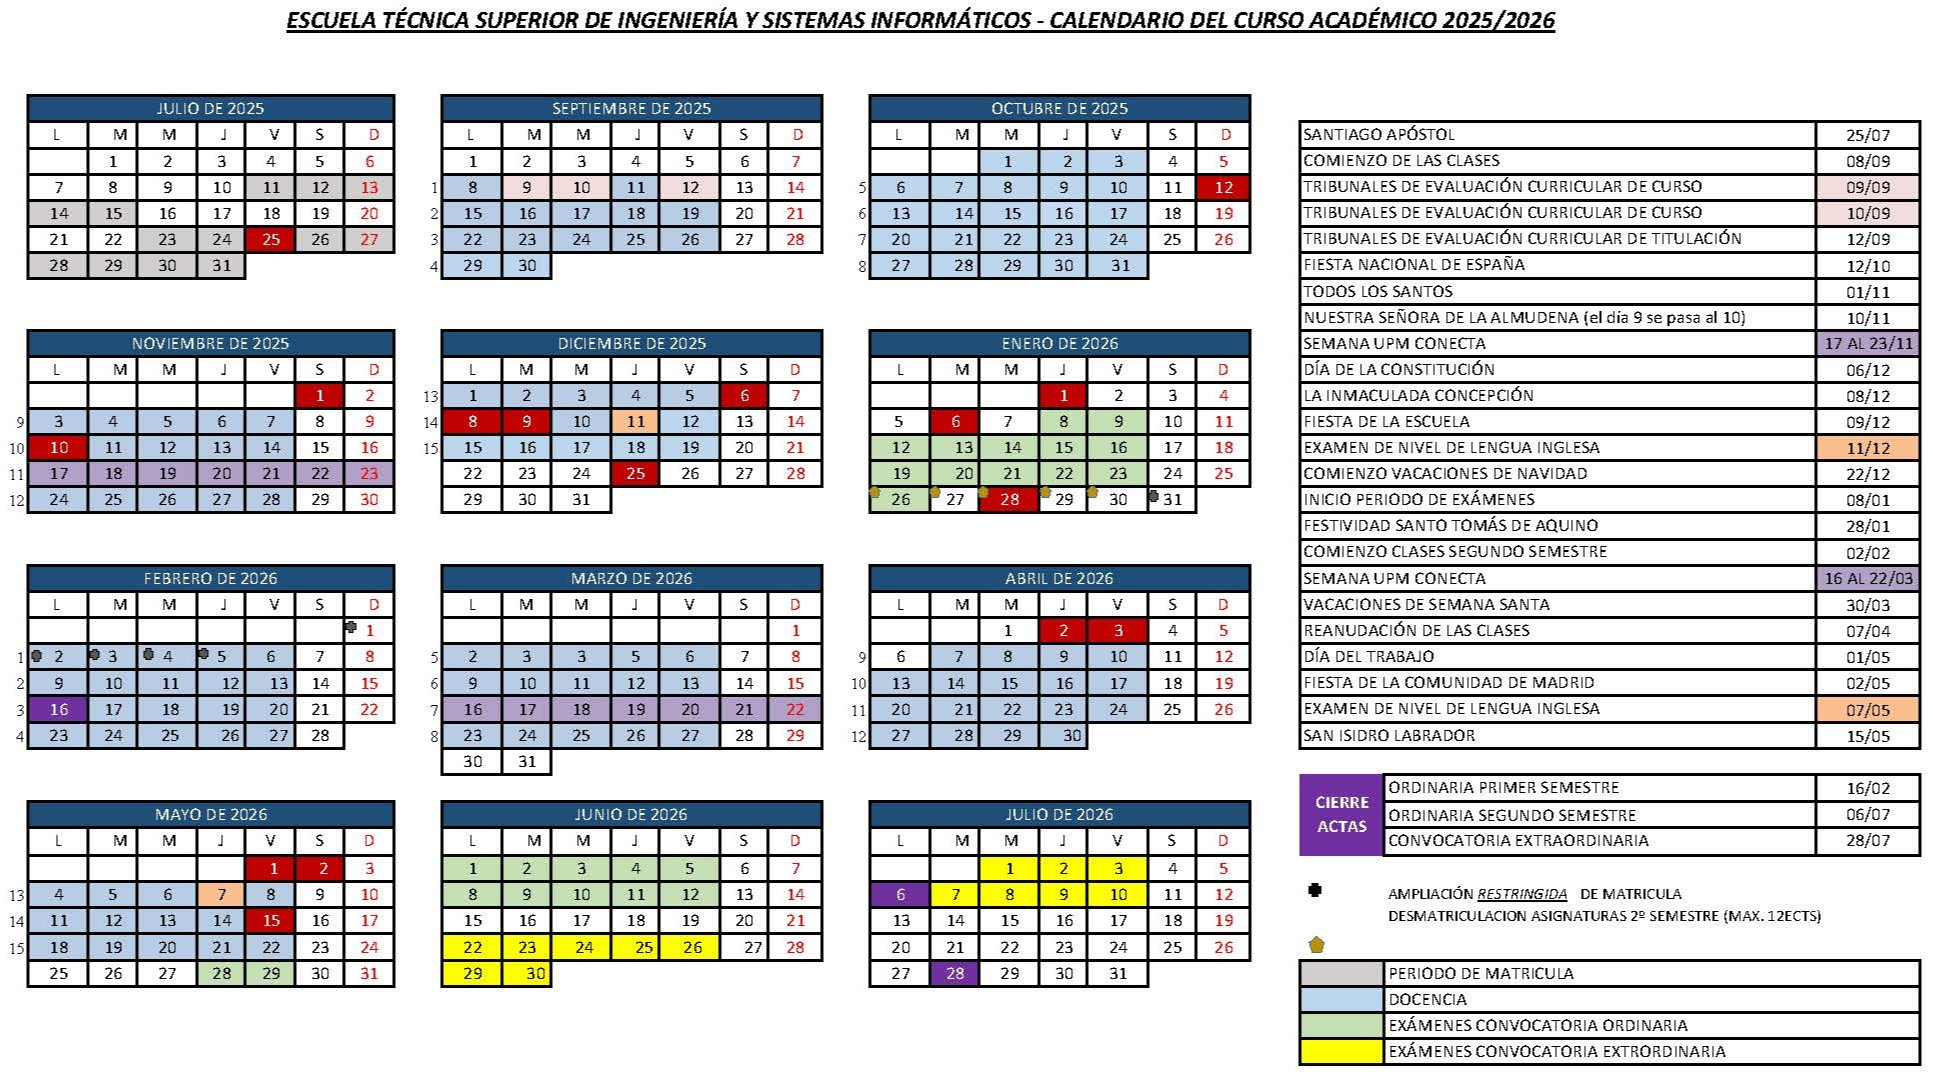
\includegraphics[width=0.8\textwidth]{Slides/figures/Presentacion/Calendario_Academico.png}
\end{figure}
\end{frame}

\begin{frame}{Calendario de sesiones (PROVISIONAL)}
\begin{figure}
    \centering
    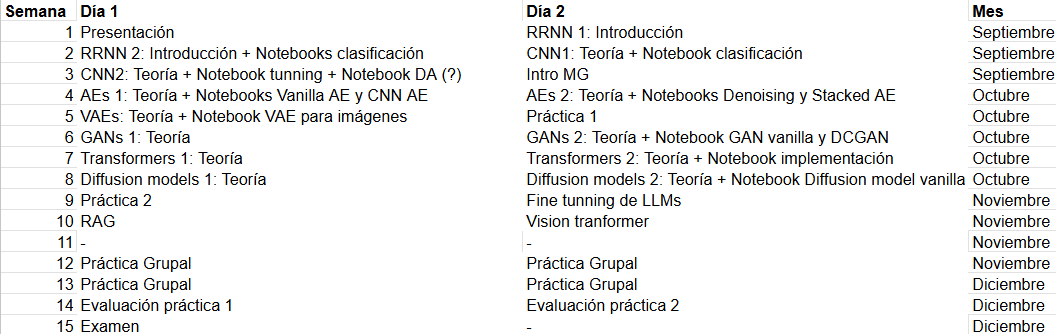
\includegraphics[width=\textwidth]{Slides/figures/Presentacion/Sesiones.png}
\end{figure}
\end{frame}

\begin{frame}{Asignaturas previas recomendadas}
\begin{itemize}
    \item \alert{Probabilidad y estadística}
    \begin{itemize}
        \item Estadística analítica
        \item Probabilidad, especialmente bayesiana
    \end{itemize}
    \item \alert{Inteligencia Artificial}
    \begin{itemize}
        \item Conocimiento básico de redes neuronales
        \item Conceptos de dataset, particionamientos de entreno, validación y test, etc.
    \end{itemize}
    \item \alert{Agentes inteligentes}
    \begin{itemize}
        \item Programación de Inteligencia Artificial en Python
        \item Uso básico de las librerías Tensorflow/Keras
        \item Conocimiento de sklearn
    \end{itemize}
\end{itemize}
\end{frame}

\begin{frame}{Otros conocimientos recomendados}
\begin{itemize}
    \item \alert{Programación en Python}
    \begin{itemize}
        \item Librerías básicas: numpy, pandas, matplotlib, seaborn
        \item Librerías de inteligencia artificial: Tensorflow/Keras, sklearn
        \item Librerías de tratamiento de imágenes: matplotlib, PIL, opencv
    \end{itemize}
    \item \alert{Idioma inglés}
    \begin{itemize}
        \item Lectura de trabajos científicos en inglés
        \item Documentación mayoritariamente en inglés
    \end{itemize}
\end{itemize}
\end{frame}

\begin{frame}{Recursos}
\begin{itemize}
    \item Diapositivas de Moodle
    \item Google Collaboratory
    \item Deep Learning Book (https://www.deeplearningbook.org/)
    \item https://www.pyimagesearch.com/blog
    \item https://machinelearningmastery.com/blog
\end{itemize}
\end{frame}

\addcontentsline{toc}{section}{Referencias}

\begin{frame}[allowframebreaks]{Referencias}
    \bibliographystyle{unsrt}
    \bibliography{Slides/references.bib}
\end{frame}

\end{document}